\lab{Facial Recognition Using Eigenfaces}{Facial Recognition Using Eigenfaces}
\label{lab:FacialRecognition}

\objective{Use the singular value decomposition to build a facial recognition system.}

Suppose we have a large database containing images of human faces.
We would like to identify people by matching their pictures to those in the database.
This task is called \emph{facial recognition}.

Facial recognition is important in law enforcement, as well as other situations. 
For example, facial recognition can be combined with video surveillance to identify when a person is not authorized to be in a location.

Humans can easily compare two face images and determine whether they belong to the same person, but automating this process is more challenging.
One technique for automated facial recognition uses \emph{eigenfaces}.

\section*{Load the Data}
Eigenfaces are an efficient way to store and query a database of face images.
As the name suggests, this method uses eigenvectors of matrices related to the collection of face images.
Essentially, the method of eigenfaces projects face images to a lower-dimensional subspace in a way that preserves their distinguishing characteristics. 
In the lower-dimensional subspace, comparing face images is much faster.

Recall that a digital image may be stored as an $m \times n$ array of pixel intensities. 
In this lab, we will store the images as $mn$-vectors by concatenating the rows of the $m \times n$ arrays.

\begin{problem}
\label{prob:getTrainingFaces}
The problems in this lab will help you write a class \li{FacialRec} to perform facial recognition. 
First we need to get a database of face images.
\begin{enumerate}
\item Download the \li{faces94} face image database found at \url{http://cswww.essex.ac.uk/mv/allfaces/faces94.html} and extract the files.
You should now have a directory named ``faces94" which contains photographs of many people, organized into folders by person.
\end{enumerate}
With this directory we can begin to write our \li{FacialRec} class. This class is outlined below.
\begin{lstlisting}
import numpy as np
from scipy import linalg as la
from os import walk
from scipy.ndimage import imread
from matplotlib import pyplot as plt
import matplotlib.cm as cm 
from random import sample

class FacialRec:
    ##########Members##########
    #   F, mu, Fbar, and U 
    ###########################
    def __init__(self,path):
        self.initFaces(path)
        self.initMeanImage()
        self.initDifferences()
        self.initEigenfaces()

    def initFaces(self, path):
        self.F = getFaces(path)
    def initMeanImage(self):
        pass
    def initDifferences(self):
        pass
    def initEigenfaces(self):
        pass
    def project(self, A, s=38):
        pass
    def findNearest(self, image, s=38):
        pass
\end{lstlisting}

The function \li{getFaces()} should construct a database of face images by selecting exactly one face image for each person in the directory.
It should return an array whose columns are the selected face images.
One implementation of this function is found at the end of this lab.

\begin{enumerate}
\item Initialize a \li{FacialRec} instance with the command \li{facialRec = FacialRec(\"./faces94\")}. You may have to replace the parameter \li{\"./faces94\"} with the location of the directory \li{faces94} on your machine. Check that \li{facialRec.F} is a $36000 \times 153$ array. The columns of this array are 153 face images of 153 different people.
\end{enumerate}
\end{problem}


\section*{Shift By the Mean}

The facial recognition algorithm is more robust if we first \emph{shift by the mean}. When we shift a set of data by the mean, the distinguishing features are exaggerated. Therefore, in the context of facial recognition, shifting by the mean accentuates the unique features of the face.
Suppose we have a collection of $k$ face images represented as vectors $\f_1, \f_2, \ldots, \f_k$ of length $mn$.
Define the \emph{mean face} ${\boldsymbol \mu}$ to be the average of the $\f_i$:
\[
{\boldsymbol \mu} = \frac{1}{k}\sum_{i=1}^k \f_i.
\]
\begin{figure}
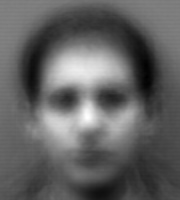
\includegraphics[width=0.3\textwidth]{meanFace.png}
\caption{The mean face.}
\label{facialRecognition:meanFace}
\end{figure}

\begin{problem}
\label{prob:meanFace}
\leavevmode
\begin{enumerate}
\item Implement the method \li{FacialRec.initMeanImage()} as follows.
\begin{lstlisting}
def initMeanImage(self):
    self.mu = # Compute the mean face of the images in self.F
\end{lstlisting}
This can be done in one line using \li{np.mean} and specifying the correct axis.

\item Plot the mean face. 
The function \li{show()} at the end of this lab will plot a flattened grayscale image.
Your mean face should match Figure \ref{facialRecognition:meanFace}.
\end{enumerate}
\end{problem}



\begin{figure}
\begin{subfigure}[b]{0.3\textwidth}
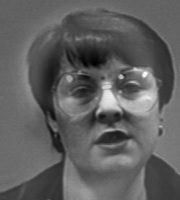
\includegraphics[width=\textwidth]{differenceFace0.png}
\end{subfigure}
\begin{subfigure}[b]{0.3\textwidth}
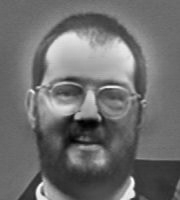
\includegraphics[width=\textwidth]{differenceFace1.png}
\end{subfigure}
\begin{subfigure}[b]{0.3\textwidth}
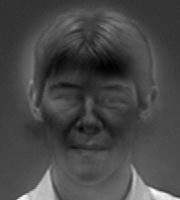
\includegraphics[width=\textwidth]{differenceFace2.png}
\end{subfigure}
\caption{Three mean-shifted faces from the dataset.}
\label{facialRecognition:differenceFaces}
\end{figure}
For each $i = 1,\ldots, k$, define $\bar{\f}_i := \f_i - {\boldsymbol \mu}$.
The mean-shifted face vector $\bar{\f}_i$ is the deviation of the $i$-th face from the mean, and thus captures the unique features of the face.
Now form the $mn \times k$ matrix $\bar{F}$ whose columns are given by the mean-shifted face vectors, i.e.
\[
\bar{F} = \begin{bmatrix}
\bar{\f}_1 & \bar{\f}_2 & \cdots & \bar{\f}_k
\end{bmatrix}.
\]
\begin{problem}
\leavevmode
\begin{enumerate}
\item Implement the method \li{FacialRec.initDifferences()} to compute $\bar{F}$ as follows.
\begin{lstlisting}
def initDifferences(self):
    self.Fbar = # Compute the mean-shifted face vectors Fbar
\end{lstlisting}
This can be done in one line using array broadcasting.
\item
Plot a mean-shifted face. The output should be similar to the faces in Figure \ref{facialRecognition:differenceFaces}.
\end{enumerate}
\end{problem}

\section*{Project to a Subspace}
Now suppose we have a new face vector $\g$. 
The closest face image to $\g$ should be the vector $\bar{\f}_i$ that minimizes $\|\bar{\g}-\bar{\f}_i\|_2$, where $\bar{\g} = \g - {\boldsymbol \mu}$.
Unfortunately, computing $\|\bar{\g}-\bar{\f}_i\|_2$ for each $i$ is computationally intractable when the length $mn$ of the vectors is large.
Since a low-resolution photo may easily have $100\times 100 = 10,000$ pixels, in practice $mn$ is very large indeed.

Here is the trick: instead of computing in the $mn$-dimensional space of all possible images, we will compute in a lower-dimensional subspace.
We could start by using the subspace spanned by the vectors $\bar{\f}_1, \ldots \bar{\f}_k$, which is at most $k$-dimensional. 
Unfortunately, in practice $k$ is still too large for this subspace to be computationally efficient.
%We need to project our problem into some subspace of the span of $\bar{\f}_1, \ldots \bar{\f}_k$.

Therefore, we want to project to a subspace of $\bar{\f}_1, \ldots \bar{\f}_k$ in a way that retains as much information about the $\bar{\f_i}$ as possible.
Mathematically, we want to find the $s$-dimensional subspace of $\text{span}\{\bar{\f}_1, \ldots \bar{\f}_k\}$ that is closest to the $\bar{\f_i}$ in the least-squares sense.
In a minute, we will prove that the SVD of $\bar{F}$ (whose columns are $\bar{\f}_1, \ldots \bar{\f}_k$) solves this problem.
But first, let us summarize how the solution works.

Let $U \Sigma V^T$ be an SVD of $\bar{F}$ with $\u_i$ the columns of $U$. 
Then the ``best'' $s$-dimensional subspace for approximating $\text{span}\{\bar{\f}_1, \ldots \bar{\f}_k\}$ is the span of $\u_1, \ldots, \u_s$. 
The matrix for this projection is $P_s = U_s U_s^T$ where $U_s = [ \u_1\; \ldots \; \u_s]$.

Because the vectors $\u_i$ are eigenvectors of $\bar{F}\bar{F}^T$, we call them \emph{eigenfaces}. 
Therefore, the best $s$-dimensional subspace for solving the facial recognition problem is exactly the span of the first $s$ eigenfaces.

\subsection*{The Proof: SVD as a Least Squares Solution}
\begin{theorem}
Let $\f_1, \ldots, \f_k$ be vectors on $\mathbb{R}^{mn}$, and let $\bar{F} = [\bar{f}_1 \; \ldots \; \bar{f}_k]$. Suppose $U\Sigma V^T$ is an SVD for $\bar{F}$. Then the $s$-dimensional subspace that solves the least squares problem for $\f_1, \ldots, \f_k$ is the span of the first $s$ columns of $U$. If $U_s$ is the first $s$ columns of $U$, then the matrix $U_sU_s^T$ is projection onto this subspace.
\end{theorem}
\begin{proof}
We seek a rank-$s$ projection matrix $P_s$ so that $\sum_{i=1}^k \|P_s\bar{\f}_i - \bar{\f}_i\|_2^2$ is minimized---i.e.,
 the sum of the squares of the ``errors'' is minimal when we project $\bar{\f}_i$ via $P_s$.
 But minimizing this quantity is the same as minimizing its square, which happens to equal the Frobenius norm of $P_s\bar{F} - \bar{F}$. 
Written mathematically,
 \begin{align*}
\inf_{\text{rank}(P_s)=s} \sum_{i=1}^k \|P_s\bar{\f}_i - \bar{\f}_i\|_2^2 &=  \inf_{\text{rank}(P_s)=s} \left( \sum_{i=1}^k \|P_s\bar{\f}_i - \bar{\f}_i\|_2^2 \right) ^2\\
 & =  \inf_{\text{rank}(P_s)=s} \| P_s\bar{F}-\bar{F}\|_F.
 \end{align*}
 
Now let $U \Sigma V^T$ be an SVD of $\bar{F}$ with $\u_i$ the columns of $U$, $\v_i$ the columns of $V$, and $\sigma_i$ the singular values of $\bar{F}$.
If $P_s = \sum_{i=1}^s \u_i \u_i^T$, then 
\begin{align*}
P_s\bar{F} &=  \left( \sum_{i=1}^s \u_i \u_i^T \right)\left(  \sum_{j=1}^k \sigma_j \u_i \v_i^T \right)
= \sum_{i=1}^s\sum_{j=1}^k \sigma_j \u_i\u_i^T\u_j\v_j^T\\
&=  \sum_{i=1}^s\sum_{j=1}^k \sigma_j \u_i\delta_{ij}\v_j^T
= \sum_{i=1}^s \sigma_i \u_i\v_i^T.
\end{align*}

In fact, the Schmidt-Eckart-Young-Mirsky Theorem from Lab \ref{lab:SVD} tells us that $X = \sum_{i=1}^s \sigma_i \u_i\v_i^T$ is exactly the rank-$s$ matrix that minimizes $\|X - \bar{F}\|_F$. 
Since $P_s \bar{F}$ will always have rank $s$ or less, the projection $P_s =  \sum_{i=1}^s \u_i \u_i^T$ is the one we seek.
If we let $U_s = [ \u_1\; \ldots \; \u_s]$, then we may write $P_s = U_sU_s^T$. Notice that $P_s$ is projection onto the subspace spanned by the columns of $U_s$.
\end{proof}

\begin{problem}
\label{prob:svd}
\leavevmode
\begin{enumerate}
\item Implement the method \li{FacialRec.initEigenfaces()} as follows.
\begin{lstlisting}
def initEigenfaces(self):
    self.U, s, Vt = # Compute the SVD of Fbar
\end{lstlisting}
This can be done in one line with the function \li{linalg.svd()}.
Because we will only use the first few columns of $U$, specify the keyword parameter \li{full_matrices=False} to compute only the compact SVD.
\item Plot the first eigenface (i.e. the first column of \li{U}).
It should match the first eigenface shown in Figure \ref{facialRecognition:eigenfaces}.
\end{enumerate}
\end{problem}

\section*{Change Basis}

It does us no good to project all our vectors into an $s$-dimensional space if we still store them as vectors in $\mathbb{R}^{nm}$. 
Instead, we must store our face vectors in terms of the columns of $U_s$.
This way, each vector is a length-$s$ array in NumPy, instead of a length-$mn$ array.

The change-of-basis matrix is $U_s^T$, so $U_s^T\widehat{P}_s = U_s^TU_sU_s^T = U_s^T$. 
Thus we can project into the subspace and change basis by multiplying by $U_s^T$.
To change back to the full $mn$-vector, multiply by $U_s$.


\begin{figure}
\begin{subfigure}[b]{0.3\textwidth}
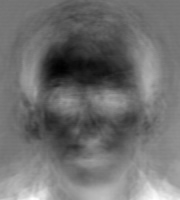
\includegraphics[width=\textwidth]{eigenface0.png}
\end{subfigure}
\begin{subfigure}[b]{0.3\textwidth}
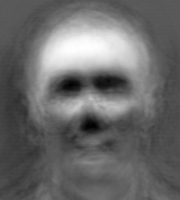
\includegraphics[width=\textwidth]{eigenface1.png}
\end{subfigure}
\begin{subfigure}[b]{0.3\textwidth}
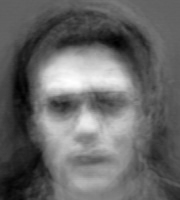
\includegraphics[width=\textwidth]{eigenface2.png}
\end{subfigure}
\caption{The top three eigenfaces.}
\label{facialRecognition:eigenfaces}
\end{figure}



\begin{problem}
\label{prob:top_n}
\leavevmode
\begin{enumerate}
\item Implement the method  \li{FacialRec.project(s)} as follows.
\begin{lstlisting}
def project(self,A,s=38):
    # project A onto s-dimensional subspace and return A_s.
\end{lstlisting}
\item (Optional) Let \li{face} be the first mean-shifted face from the database (the first column of \li{facialRec.Fbar}). Do the following:
\begin{enumerate}
\item Project \li{face} onto the subspace spanned by the first 75 eigenfaces.
\item Change basis back to the standard basis on $\mathbb{R}^{mn}$.
\item Add back the mean face \li{facialRec.mu}.
\item Plot the resulting image.
\end{enumerate}
Your image should match Figure \ref{fig:75_efaces}.
\end{enumerate}
\end{problem}


\begin{figure}

\begin{subfigure}[b]{0.3\textwidth}
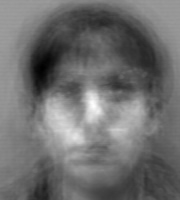
\includegraphics[width=\textwidth]{rebuiltThirtySecond.png}
\caption{5 eigenfaces, about 1/32 of the total.}
\label{fig:5_efaces}
\end{subfigure}
\begin{subfigure}[b]{0.3\textwidth}
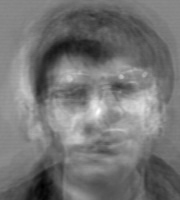
\includegraphics[width=\textwidth]{rebuiltSixteenth.png}
\caption{9 eigenfaces, or 1/16 of the total.}
\label{fig:9_efaces}
\end{subfigure}
\begin{subfigure}[b]{0.3\textwidth}
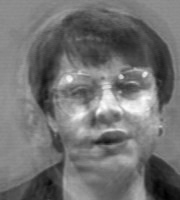
\includegraphics[width=\textwidth]{rebuiltEighth.png}
\caption{19 eigenfaces, about 1/8 of the total.}
\label{fig:19_efaces}
\end{subfigure}
\begin{subfigure}[b]{0.3\textwidth}
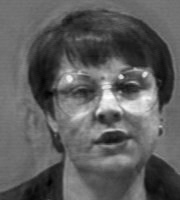
\includegraphics[width=\textwidth]{rebuiltFourth.png}
\caption{38 eigenfaces, about 1/4 of the total.}
\label{fig:38_efaces}
\end{subfigure}
\begin{subfigure}[b]{0.3\textwidth}
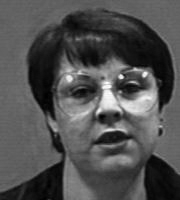
\includegraphics[width=\textwidth]{rebuiltHalf.png}
\caption{75 eigenfaces, about 1/2 of the total.}
\label{fig:75_efaces}
\end{subfigure}
\begin{subfigure}[b]{0.3\textwidth}
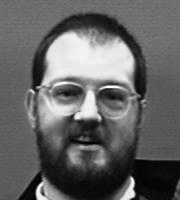
\includegraphics[width=\textwidth]{rebuiltAll.png}
\caption{All 153 of the eigenfaces.}
\label{fig:all_efaces}
\end{subfigure}
\caption{Image rebuilt with various numbers of eigenfaces. The image is somewhat recognizable when it is reconstructed with only 1/8 of the eigenfaces.}
\label{fig:rebuiltImage}
\end{figure}

\begin{comment}
Of course, moving to a lower-dimensional subspace by using only the top $n$ eigenfaces introduces some error, in the sense that we cannot perfectly
reconstruct the face images from their coordinate vectors.
However, this error is tolerable, provided $n$ is not \emph{too} small.
Note that we can approximately reconstruct $\bar{f}_i$ from the coordinate vector $\hat{f}_i$ by
\[
\bar{f}_i \approx U_n\hat{f}_i.
\]
See Figure \ref{facialRecognition:rebuiltImage} for examples of reconstructed face images giving different numbers of eigenfaces.
\end{comment}

\section*{Recognizing Faces}
Finally, we are ready to identify which mean-shifted image $\bar{\f}_i$ is closest to an inputed image, $\bar{\g}$. 
We begin by projecting all vectors to some $s$-dimensional subspace and writing them in terms of an orthonormal basis for that subspace. 
This is accomplished with multiplication by $U_s^T$:
\[
\widehat{\f}_i = U_s^T(\f_i-{\boldsymbol \mu}) \qquad \widehat{\g} = U_s^T(\g-{\boldsymbol \mu}).
\]

Next, we compute which $\widehat{\f}_i$ is closest to $\widehat{\g}$. 
Since the columns of $U_s$ are an orthonormal basis, we get the same result doing the computation in this basis as we would in the standard Euclidean basis.
Define
\[
i^* = \text{argmin}_i \|\widehat{\f}_i - \widehat{\g}\|_2.
\]
Then the $i^*$-th face image is the best match for $\g$.

\begin{problem}
\label{prob:nearest}
\leavevmode
\begin{enumerate}
\item
Implement the method \li{FacialRec.findNearest()} as follows.
\begin{lstlisting}
def findNearest(self, image, s=38):
    Fhat = # Project Fbar, producing a matrix whose columns are the f-hat defined above 
    ghat = # Shift 'image' by the mean and project, producing g-hat as defined above
    # for both Fhat and ghat, use your project function from the previous problem
    
    # Return the index that minimizes ||fhat_i - ghat||_2.
\end{lstlisting}
The functions \li{np.linalg.norm()} and \li{np.argmin()} will be useful for the last line. When using \li{np.linalg.norm}, make sure you indicate the correct axis. 

\item Test your facial recognition system on faces selected randomly from the \li{faces94} dataset.
The function \li{sampleFaces(n_tests, path)} at the end of this lab will build an array of \li{n_tests} random faces from the \li{faces94} database.

Plot the random face beside the face returned by your facial recognition code to see if your system is accurately recognizing faces.
The function \li{show2()} at the end of this lab will plot two face vectors side-by-side.

\end{enumerate}
\end{problem}


By this point, you have created a basic facial recognition system.
We can extend the system to detect when a face doesn't match anything currently in the database, and then add this new face into the database.
We can also make the system more robust by including multiple pictures of the same face with different expressions and lighting conditions.

Although there are other approaches to facial recognition that utilize more complex techniques, the method of eigenfaces remains
a wonderfully simple and effective solution, illustrating another application of the singular value decomposition.

\section*{Appendix: Helper Code}
This section contains some functions to help you code up the facial recognition class outlined in the problems of this lab.

\begin{lstlisting}
def getFaces(path="./faces94"):
    """Traverse the directory specified by 'path' and return an array containing
    one column vector per subdirectory.
    
    For the faces94 dataset, this gives an array with just one column for each
    face in the database. Each column corresponds to a flattened grayscale image.
    """
    
    # Traverse the directory and get one image per subdirectory.
    faces = []
    for (dirpath, dirnames, filenames) in walk(path):
        for f in filenames:
            if f[-3:]=="jpg": # only get jpg images
                # load image, convert to grayscale, flatten into vector
                face = imread(dirpath+"/"+f).mean(axis=2).ravel() 
                faces.append(face)
                break
        
    # put all the face vectors column-wise into a matrix.
    F = np.array(faces).T
    return F


def show(im, w=200, h=180):
    """Plot the flattened grayscale image 'im' of width 'w' and height 'h'."""
    
    plt.imshow(im.reshape((w,h)), cmap=cm.Greys_r)
    plt.show()
    


def sampleFaces(n_tests,path = "./faces94")
    """Return an array containing a sample of n_tests images contained 
    in the path as flattened images in the columns of the output.
    """
    files = []
    for (dirpath, dirnames, filenames) in walk(path):
        for f in filenames:
            if f[-3:]=="jpg": # only get jpg images
            files.append(dirpath+"/"+f)
            
    #Get a sample of the images
    test_files = sample(files, n_tests)
    #Flatten and average the pixel values
    images = np.array([imread(f).mean(axis=2).ravel() for f in test_files]).T
    return images
    

def show2(im1, im2, w=200, h=180):
    """Convenience function for plotting two flattened grayscale images of
    the specified width and height side by side.
    """
    plt.subplot(121)
    plt.imshow(im1.reshape((w,h)), cmap=cm.Greys_r)
    plt.subplot(122)
    plt.imshow(im2.reshape((w,h)), cmap=cm.Greys_r)
    plt.show()


\end{lstlisting}
